\documentclass[12pt]{article}

\usepackage{fullpage}
\usepackage{multicol,multirow}
\usepackage{tabularx}
\usepackage{ulem}
\usepackage[utf8]{inputenc}
\usepackage[russian]{babel}
\usepackage{amsmath}
\usepackage{amssymb}
\usepackage{graphicx}
\graphicspath{./}
\usepackage{color}
\usepackage{titlesec}

\titleformat{\section}
  {\normalfont\Large\bfseries}{\thesection.}{0.3em}{}

\titleformat{\subsection}
  {\normalfont\large\bfseries}{\thesubsection.}{0.3em}{}

\titlespacing{\section}{0pt}{*2}{*2}
\titlespacing{\subsection}{0pt}{*1}{*1}
\titlespacing{\subsubsection}{0pt}{*0}{*0}
\usepackage{listings}
\lstloadlanguages{Lisp}
\lstset{extendedchars=false,
	breaklines=true,
	breakatwhitespace=true,
	keepspaces = true,
	tabsize=2
}
\begin{document}


\section*{Отчет по лабораторной работе №\,4
по курсу \guillemotleft  Функциональное программирование\guillemotright}
\begin{flushright}
Студент группы 8О-308 МАИ \textit{Балес Александр}, \textnumero 3 по списку \\
\makebox[7cm]{Контакты: {\tt aleks\_bales@mail.ru} \hfill} \\
\makebox[7cm]{Работа выполнена: 21.05.2016 \hfill} \\
\ \\
Преподаватель: Иванов Дмитрий Анатольевич, доц. каф. 806 \\
\makebox[7cm]{Отчет сдан: \hfill} \\
\makebox[7cm]{Итоговая оценка: \hfill} \\
\makebox[7cm]{Подпись преподавателя: \hfill} \\

\end{flushright}

\section{Тема работы}
Знаки и строки.

\section{Цель работы}
Научиться работать с литерами (знаками) и строками при помощи функций обработки строк и общих функций работы с последовательностями.

\section{Задание(вариант 4.34)}
Запрограммировать на языке Коммон Лисп функцию \tt{find-word}, принимающую два аргумента:
\begin{itemize}
\item word - строка, представляющая слово,
\item source - текст.
\end{itemize}
Если слово найдено, функция должна возвращать два значения с помощью \tt{values}:
\begin{enumerate}
\item индекс начала данного слова в предложении,
\item номер первого предложения в тексте, в которое входит слово (нумерация с 0). 
\end{enumerate}
Если слово не найдено, функция должна вернуть NIL.

\section{Оборудование студента}
Процессор Intel Core i5-3210 4\,@\,2.5GHz, память: 8192Mb, разрядность системы: 64.

\section{Программное обеспечение}
ОС Ubuntu 14.04, среда GNU Common Lisp 2.6.10

\section{Идея, метод, алгоритм}
Получаем из текста список слов, обходим этот список слов в цикле \tt{for}, сравниваем два слова:
\begin{enumerate}
\item сравниваем по символьно два слова, от $0$ до $n$, где $n = min(len(s1), len(s2))$
\item если в ходе сравнений различия не обнаружились, то необходимо сравнить длины обох слов
\item если длины отличаются на 1, и крайний символ в \tt{s2} является одним из разделителей в предложении, тогда строки равны
\item иначе не равны
\end{enumerate}
\section{Сценарий выполнения работы}
\section{Распечатка программы и её результаты}
\lstinputlisting{./lr4.lsp}
\subsection{Результаты}
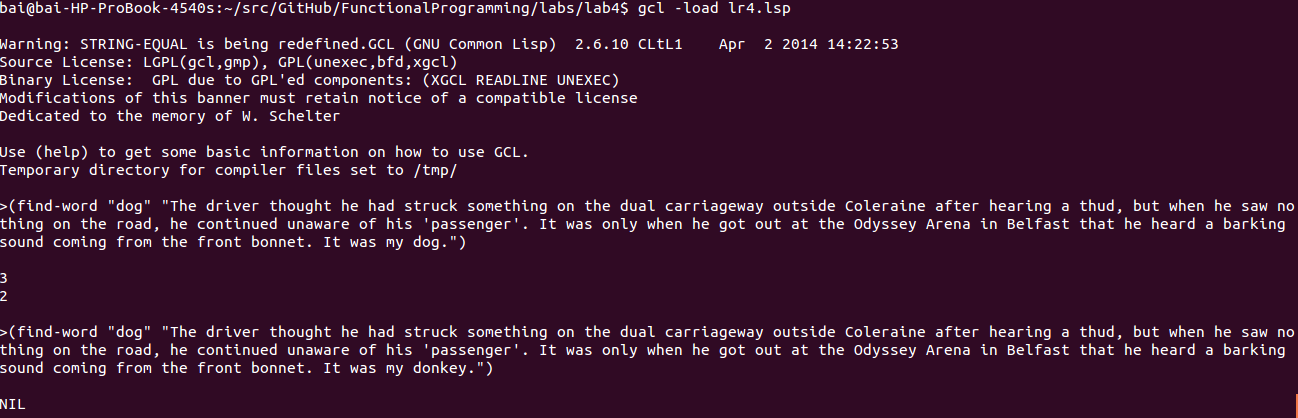
\includegraphics[scale=0.5]{lr4Screen}

%\subsection{Результаты работы}
%\lstinputlisting{./log2.lsp}

\section{Дневник отладки}
\begin{tabular}{|c|p{5cm}|p{5cm}|p{3cm}|}
\hline
Дата & Событие & Действие по исправлению & Примечание \\
\hline
25.05.2016 & BugFix & Исправил функцию сравнения строк, т.к. она работала некорректно, воспользовался стандартной {\color{red}\tt{string-equal}} & Пришлось написать парсер, который отбросит точки и запятые в слове, для корректного сравнения с {\color{blue}\tt{word}}\\
\hline 
\end{tabular}

\section{Замечания, выводы}
Я научился работать с литерами (знаками) и строками при помощи функций обработки строк и общих функций работы с последовательностями.
\end{document}
